\
\documentclass[usenames,dvipsnames]{beamer}
\mode<presentation>{\usetheme{Warsaw}}
\usepackage{textpos} %package for text positioning

%%%%%%%%%%%%%%%%%%%%%%%%%%%%%%%%%%%%%%%%%%%%%%%%%%%%%%%%%%%%%%%%%%%%%%%%%%%%%%%%%%%%
%Normal Math Packages
\usepackage{amsmath}
\usepackage{amsfonts}
\usepackage{enumerate}
\usepackage{amsmath}
\usepackage{mathtools}
\usepackage{tikz-cd}
\usepackage{ragged2e}
\usepackage{mathrsfs}
%%%%%%%%%%%%%%%%%%%%%%%%%%%%%%%%%%%%%%%%%%%%%%%%%%%%%%%%%%%%%%%%%%%%%%%%%%%%%%%%%%%%

%%%%%%%%%%%%%%%%%%%%%%%%%%%%%%%%%%%%%%%%%%%%%%%%%%%%%%%%%%%%%%%%%%%%%%%%%%%%%%%%%%%%
%Created Commands
\theoremstyle{definition}
\newtheorem*{remark}{Remark}
\newtheorem*{question}{Question}
%\newtheorem*{definition}{Definition}
%\newtheorem*{definitions}{Definitions}

\theoremstyle{theorem}
\newtheorem*{proposition}{Proposition}
\newtheorem*{axiom}{Axiom}

\newcommand{\R}{\mathbb{R}}
\newcommand{\Q}{\mathbb{Q}}
\newcommand{\F}{\mathbb{F}}
\newcommand{\A}{\mathcal{A}}
\newcommand{\N}{\mathbb{N}}
\newcommand{\C}{\mathbb{C}}
\newcommand{\opO}{\mathcal{O}}
\newcommand{\states}{\mathcal{S}}
%%%%%%%%%%%%%%%%%%%%%%%%%%%%%%%%%%%%%%%%%%%%%%%%%%%%%%%%%%%%%%%%%%%%%%%%%%%%%%%%%%%%


%%%%%%%%%%%%%%%%%%%%%%%%%%%%%%%%%%%%%%%%%%%%%%%%%%%%%%%%%%%%%%%%%%%%%%%%%%%%%%%%%%%%
%Stuff to make things look good
% Color modification
\setbeamercolor{structure}{fg=green!30!black}% to modify  immediately all palettes
\setbeamercolor{title}{fg=white}
\setbeamercolor{title in head/foot}{fg=yellow}

%Size Modification
\setbeamerfont{frametitle}{size=\small}

% position the logo
\addtobeamertemplate{frametitle}{}{%
\begin{textblock*}{1cm}(\textwidth,-1.1cm)

\includegraphics[height=.9cm,width=.9cm,keepaspectratio]{Lagrangian_Mechanics/csu.png}
\end{textblock*}}

% Text Positioning
\usepackage[absolute,overlay]{textpos}
%%%%%%%%%%%%%%%%%%%%%%%%%%%%%%%%%%%%%%%%%%%%%%%%%%%%%%%%%%%%%%%%%%%%%%%%%%%%%%%%%%%%

%Font
%\fontfamily{cmr}\selectfont
\usefonttheme{serif}

%Colors and stuf
\usepackage{color, soul, xcolor} % Colored text and highlighting, respectively
\usepackage{tikz-cd} % For commutative diagrams

%% preamble
\title{Lagrangian Mechanics:}
\subtitle{Math 620 Project}
\author{Colin Roberts}

\begin{document}

%%Title Frame
{
\setbeamertemplate{headline}{}
\addtobeamertemplate{frametitle}{\vspace*{-0.9\baselineskip}}{}
\begin{frame}
\titlepage
\end{frame}
}


\AtBeginSection[]
{
	\begin{frame}{Table of Contents}
		\tableofcontents[currentsection]
	\end{frame}
}
%%%%%%%%%%%%%%%%%%%%%%%%%%%%%%%%%%%%%%%%%%%%%%%%%%%%%%%%%%%%%%%%%%%%%%%%%%%%%%%
%%%%%%%%%%%%%%%%%%%%%%%%%%%%%%%%%%%%%%%%%%%%%%%%%%%%%%%%%%%%%%%%%%%%%%%%%%%%%%%
\section{Overview}
    
    
    \subsection{Mechanics}
    
        \begin{frame}{Newtonian Mechanics}
            For a system of $n$ particles (indexed by $i$), we have the following relationship:
                \[
                \dot{\mathbf{p}}_i(t)=\sum_{j}\mathbf{F}_{ij}(\mathbf{x}_1(t),\dots,\mathbf{x}_n(t),t),
                \]
            Where $j$ indexes the external forces acting on particle $i$.
            
            Usually, we assume constant mass, and we arrive at
                \[
                m_i \mathbf{\ddot{x}}_i(t)= \dot{\mathbf{p}}_i(t)
                \]
            In other words,
                \[
                m\mathbf{a}=\mathbf{F}
                \]
            holds for each particle.
        \end{frame}
        
        \begin{frame}{Potentials}
            Often times we are provided a potential as opposed to a force.  We'll denote a potential by $U(\mathbf{x})$ for a single particle system. Then Newton's laws are
            \[
            m\ddot{\mathbf{x}}=-\frac{\partial U}{\partial \mathbf{x}}=-\nabla U.
            \]
            The notation is really saying
            \[
            -\frac{\partial U}{\partial \mathbf{x}}=
            \left( -\frac{\partial U}{\partial \mathbf{x}_1},\dots,-\frac{\partial U}{\partial \mathbf{x}_n}\right)
            \]
            where $\mathbf{x}_i$ are components to some coordinate choice.
            
        \end{frame}
        
        \begin{frame}{Motivation for a New Approach}
            Consider the following:
            \begin{figure}
                \centering
                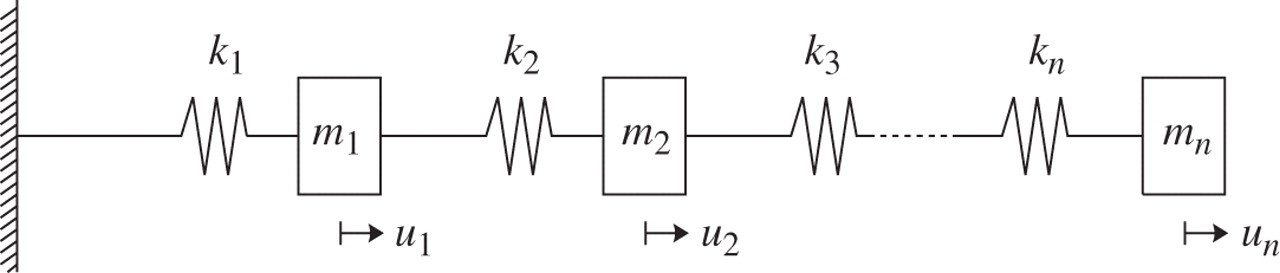
\includegraphics[width=0.9\textwidth]{Lagrangian_Mechanics/n_spring_mass.jpg}
                \caption{A system with $n$ springs and $n$ masses.}
                \label{fig:my_label}
            \end{figure}
            Now draw the free body diagram and write down $m\mathbf{a}=\mathbf{F}$ for each component and solve the system.
        \end{frame}
        
        \begin{frame}{Motivation for a New Approach}
            Let us not dive down that rabbit hole.  It ends up being extremely tedious!\\
            \vspace{.5cm}
            \noindent Instead, let us approach this via a variational method called \emph{Lagrangian Mechanics}.\\
            \vspace{.5cm}
            We'll also find other benefits from this method.
        \end{frame}
        
    \subsection{Lagrangian Mechanics}    
        
        \begin{frame}{Lagrangian Mechanics}
            \textbf{Outline:}
            \begin{itemize}
                \item Generalized Coordinates, $\mathbf{q}_i\in M$ and $\dot{\mathbf{q}_i}$.
                \item Configuration Space, $TM$.
                \item Lagrangian Function, $\mathcal{L}\colon TM \to \R$ by $\mathcal{L}=T-U$.
                \item Action Functional, $S\colon \{\textrm{Curves on $TM$}\} \to \R$.
                \item Euler-Lagrange Equations, $\displaystyle{\frac{d}{dt}\frac{\partial \mathcal{L}}{\partial \dot{\mathbf{q}_i}}-\frac{\partial \mathcal{L}}{\partial \mathbf{q}_i}=0}$, geodesics on $TM$.
            \end{itemize}
        \end{frame}
    
        \begin{frame}{Generalized Coordinates}
            \begin{figure}
                \centering
                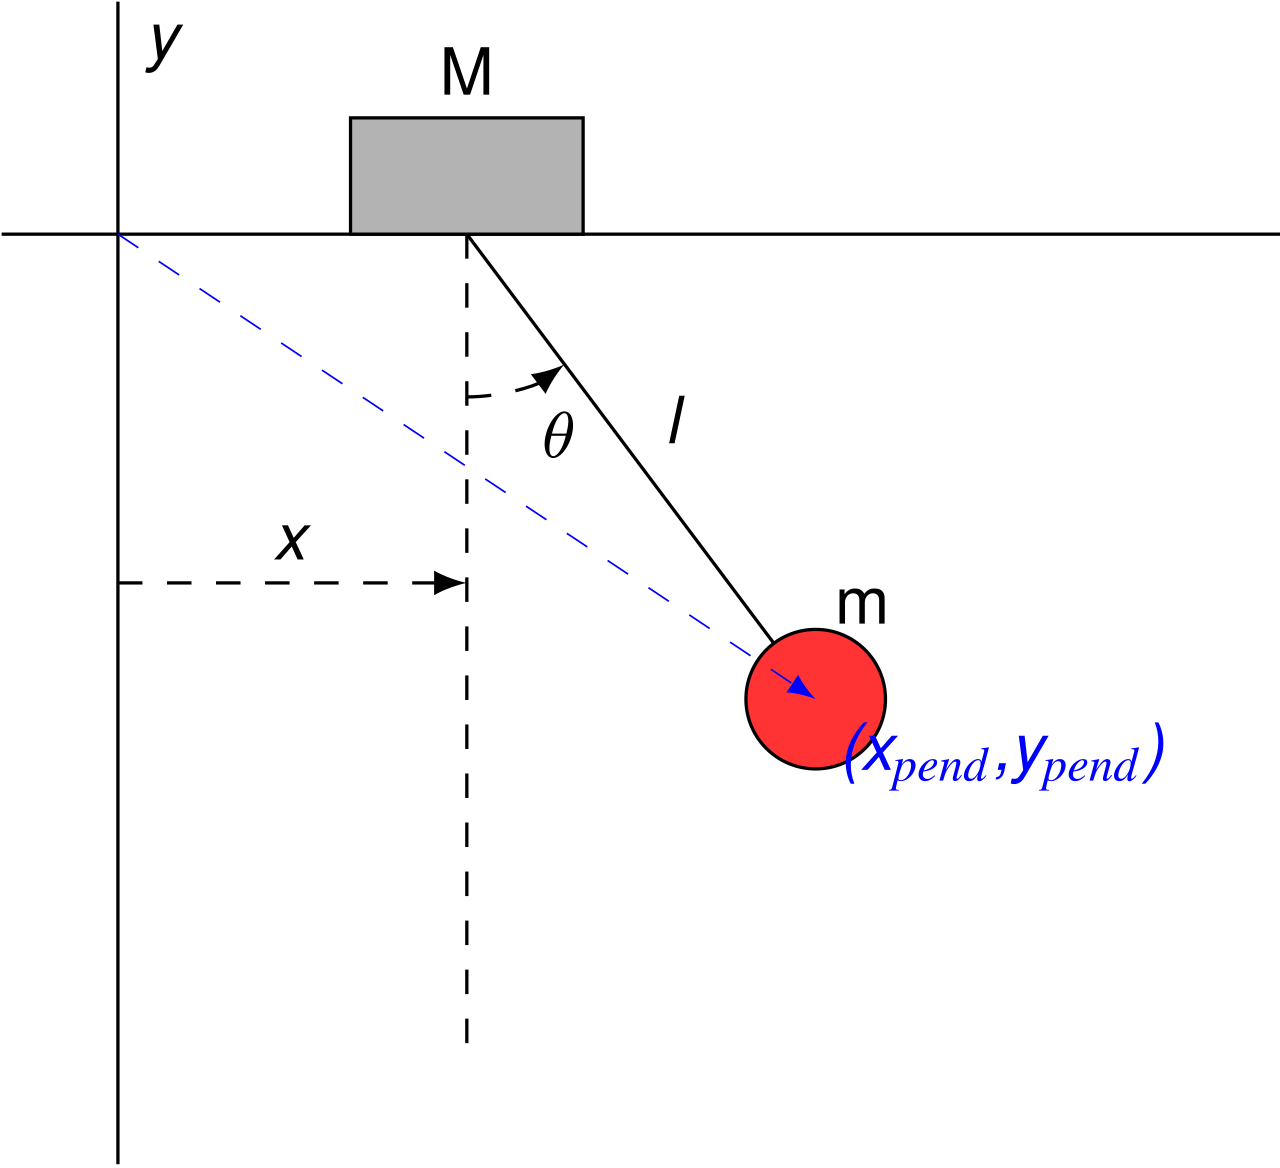
\includegraphics[width=.6\textwidth]{Lagrangian_Mechanics/generalized_coordinates.png}
                \caption{A rough picture of general coordinates in one dimension.}
                \label{fig:my_label}
            \end{figure}
        \end{frame}
        
        \begin{frame}{Generalized Coordinates}
            \begin{textblock*}{6cm}(5cm,-2cm)
            \begin{itemize}
                \item Notice first that we have two particles (masses) each moving in 1-dimension.
                \item We define:
                    \begin{align*}
                        \mathbf{q}_1(t)&=x(t),\\
                        \mathbf{\dot{q}}_1(t)&=\dot{x}(t),\\
                        \mathbf{q}_2(t)&=\theta(t),\\
                        \dot{\mathbf{q}}_2&=\dot{\theta}(t),
                    \end{align*}
                    as our generalized coordinates.
            \end{itemize}
            \end{textblock*}
            \begin{textblock*}{5cm}(0cm,-2.5cm)
            \begin{figure}
                \centering
                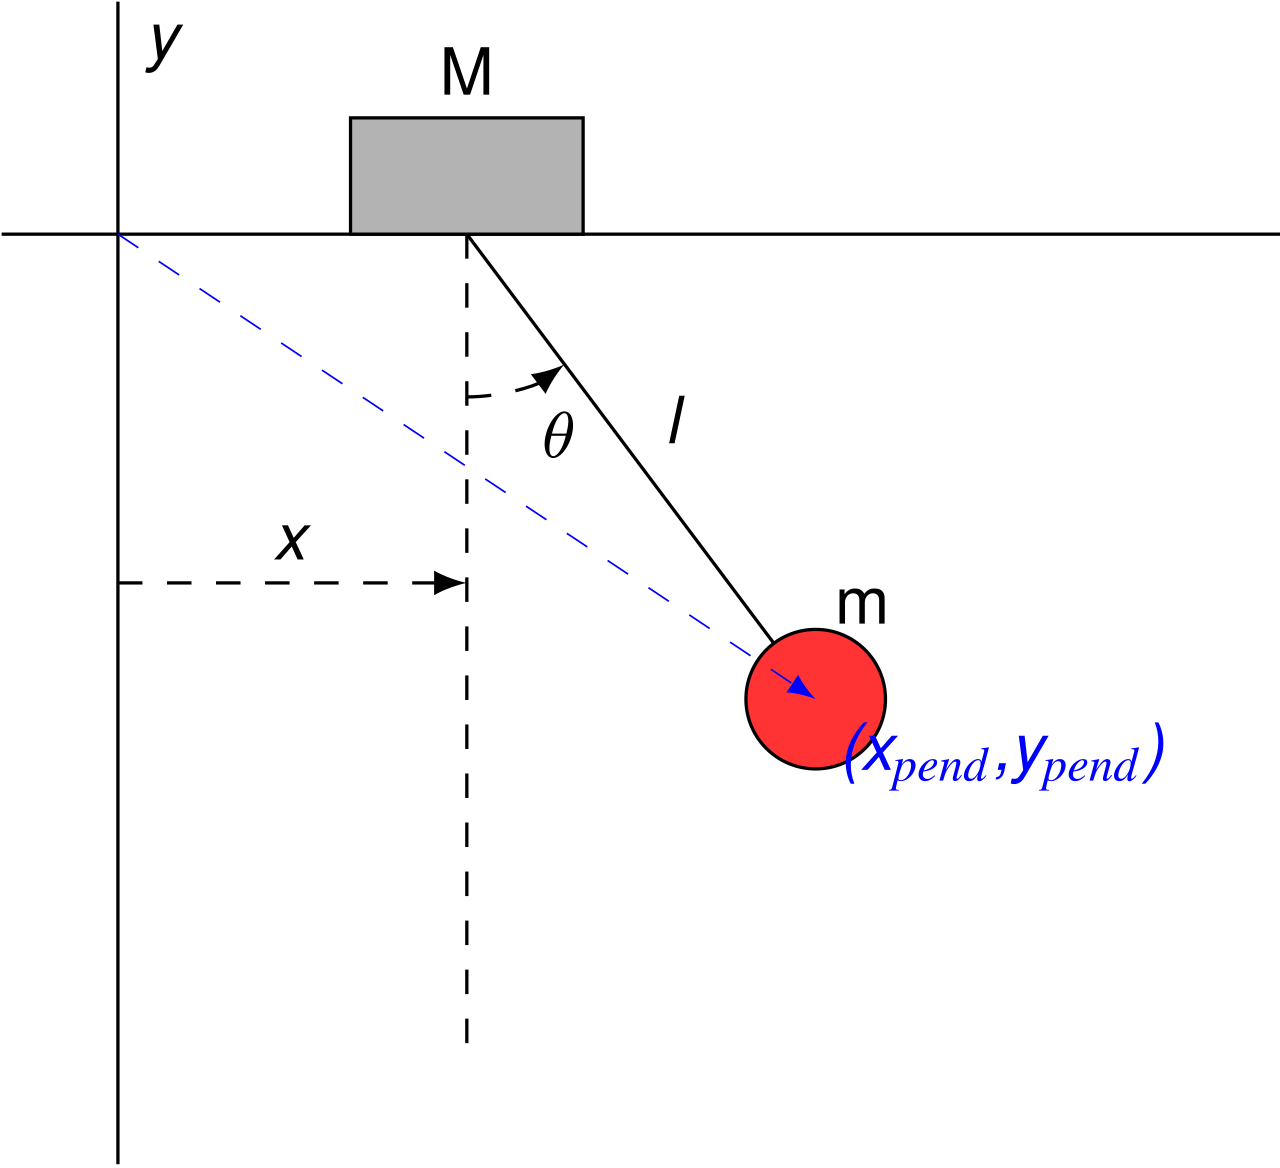
\includegraphics[width=5cm]{Lagrangian_Mechanics/generalized_coordinates.png}
                \caption{Mass $M$ has relevant coordinates in $x$, and mass $m$ has relevant coordinates in $\theta$.}
                \label{fig:my_label}
            \end{figure}
            \end{textblock*}
        \end{frame}
        
        \begin{frame}{Lagrangian Function}
            \begin{definition}
                The \emph{Lagrangian} $\mathcal{L}$ is defined to be
                \[
                \mathcal{L}(\mathbf{q}_1,\dots,\mathbf{q}_n,\mathbf{\dot{q}}_1,\dots,\mathbf{\dot{q}}_n,t)\coloneqq T-U,
                \]
                where $T(\mathbf{q}_1,\dots,\mathbf{q}_n,\mathbf{\dot{q}}_1,\dots,\mathbf{\dot{q}}_n,t)$ is the kinetic energy of the whole system, and $U(\mathbf{q}_1,\dots,\mathbf{q}_n)$ the potential energy of the whole system.
            \end{definition}
        \end{frame}
        
        \begin{frame}{Why $T-U$?}
            This begs the question, ``Why is $\mathcal{L}=T-U$?" We can prove why this is the case in a moment. We need a few more tools.
        \end{frame}
        
        \begin{frame}{Action Functional}
            \begin{definition}
                The \emph{action} $S$ is defined to be
                \[
                S\coloneqq \int_{t_1}^{t_2}\mathcal{L}dt.
                \]
            \end{definition}
        \end{frame}
        
        \begin{frame}{Euler-Lagrange Equations}
            Exactly as done in class, we look for a stationary point of the action and arrive at the Euler-Lagrange equations:
            \[
            \frac{\partial \mathcal{L}}{\partial \mathbf{q}_j}-\frac{d}{dt}\frac{\partial \mathcal{L}}{\partial \dot{\mathbf{q}}_j}=0.
            \]
        \end{frame}
        
        \begin{frame}{Euler-Lagrange to Newton}
            \begin{proof}
                For a mechanical system with one particle, we have $U(\mathbf{q})$ and $T=\frac{1}{2}m\mathbf{\dot{q}}^2$.  Then $\mathcal{L}=T-U$ so we have
                \begin{align*}
                \frac{d}{dt}\frac{\partial \mathcal{L}}{\partial \mathbf{\dot{q}}}&=\frac{d}{dt}m\mathbf{\dot{q}}\\
                &= \dot{m}\mathbf{\dot{q}}+m\mathbf{\ddot{q}}.
                \end{align*}
                Also,
                \begin{align*}
                    \frac{\partial \mathcal{L}}{\partial \mathbf{q}}=-\frac{\partial U}{\partial \mathbf{q}}.
                \end{align*}
                Setting the above equal is exactly Newton's laws!
            \end{proof}
        \end{frame}
    
        \begin{frame}{Example Problem}
            \begin{figure}
                \centering
                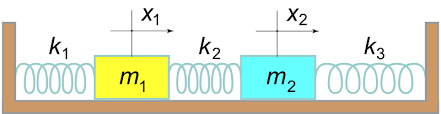
\includegraphics[width=.95\textwidth]{Lagrangian_Mechanics/2mass_3spring.png}
                \caption{Our working example.}
                \label{fig:my_label}
            \end{figure}
        \end{frame}
        
        \begin{frame}{Example Problem}
            \begin{figure}[h]
                \centering
                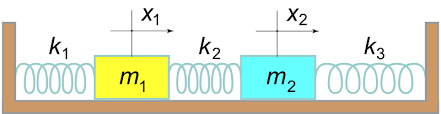
\includegraphics[width=.5\textwidth]{Lagrangian_Mechanics/2mass_3spring.png}
            \end{figure}
            First,
            \[
            T=\frac{1}{2}m_1\dot{x}_1+\frac{1}{2}m_2\dot{x}_2.
            \]
            We measure $x_1$ and $x_2$ from rest lengths of the springs and assume Hooke's law for small oscillations for the springs giving
            \[
            U=\frac{1}{2} k_1x_1^2+\underbrace{\frac{1}{2}k_2(x_2-x_1)^2}_{\textrm{interaction term}}+\frac{1}{2}x_2^2.
            \]
        \end{frame}
        
        \begin{frame}{Example Problem}
            We get the system of second order ODEs:
            \[
            \frac{d}{dt}\frac{\partial \mathcal{L}}{\partial \dot{x}_1}= \frac{\partial \mathcal{L}}{\partial x_1} \implies m_1\ddot{x}_1=-k_1x_1+k_2(x_2-x_1)
            \]
            and
            \[
            \frac{d}{dt}\frac{\partial \mathcal{L}}{\partial \dot{x}_2}= \frac{\partial \mathcal{L}}{\partial x_2} \implies m_2\ddot{x}_2=-k_2(x_2-x_1)-k_3x_2.
            \]
            The interaction term before couples these equations.
        \end{frame}
        
        \begin{frame}{Example Problem}
            This is a problem we can solve using techniques from Math 340.  We create new variables, $\dot{x}_1=y_1$ and $\dot{x}_2=y_2$ and we can write
            \[
            \begin{bmatrix}
            \dot{x}_1\\
            \dot{y}_1\\
            \dot{x}_2\\
            \dot{y}_2
            \end{bmatrix}
            =
            \begin{bmatrix}
            0 & 1 & 0 & 0\\
            \frac{-2k}{m} & 0 & \frac{k}{m} & 0\\
            0 & 0 & 0 & 1\\
            \frac{k}{m} & 0 & \frac{-2k}{m} & 0
            \end{bmatrix}
            \begin{bmatrix}
            x_1\\
            y_1\\
            x_2\\
            y_2
            \end{bmatrix}.
            \]
            The eigenvalues are $\pm i\sqrt{\frac{k}{m}}$, and $\pm i\sqrt{\frac{3k}{m}}.$
        \end{frame}
        
        \begin{frame}{Example Problem}
            Visualization of fundamental modes.
            https://www.math24.net/mass-spring-system/\\
            
            \vspace{.5cm}
            These fundamental modes are important in physical theories like particle physics.
        \end{frame}
        
\section{Further Concepts}

        
    \subsection{Potentials}
        
        \begin{frame}{Stationary Points Versus Minimizers}
            We can rephrase a theorem from class:
            \begin{theorem}
            Let $\Omega \subseteq \R$ be connected and open, and $\mathcal{L}\in C^0(\overline{\Omega}\times \R \times \R)$ with $(\mathbf{q},\dot{\mathbf{q}})\mapsto \mathcal{L}(t,\mathbf{q},\dot{\mathbf{q}})$ strictly convex. Then 
            \[
            S=\int_{t_1}^{t_2} \mathcal{L}(t,\mathbf{q},\dot{\mathbf{q}})d\mathbf{t}
            \]
            has a unique minimizer.
            \end{theorem}
        \end{frame}
        
        \begin{frame}{Symmetry Breaking}
            When potentials are not convex, very interesting things can happen!
            \begin{figure}
                \centering
                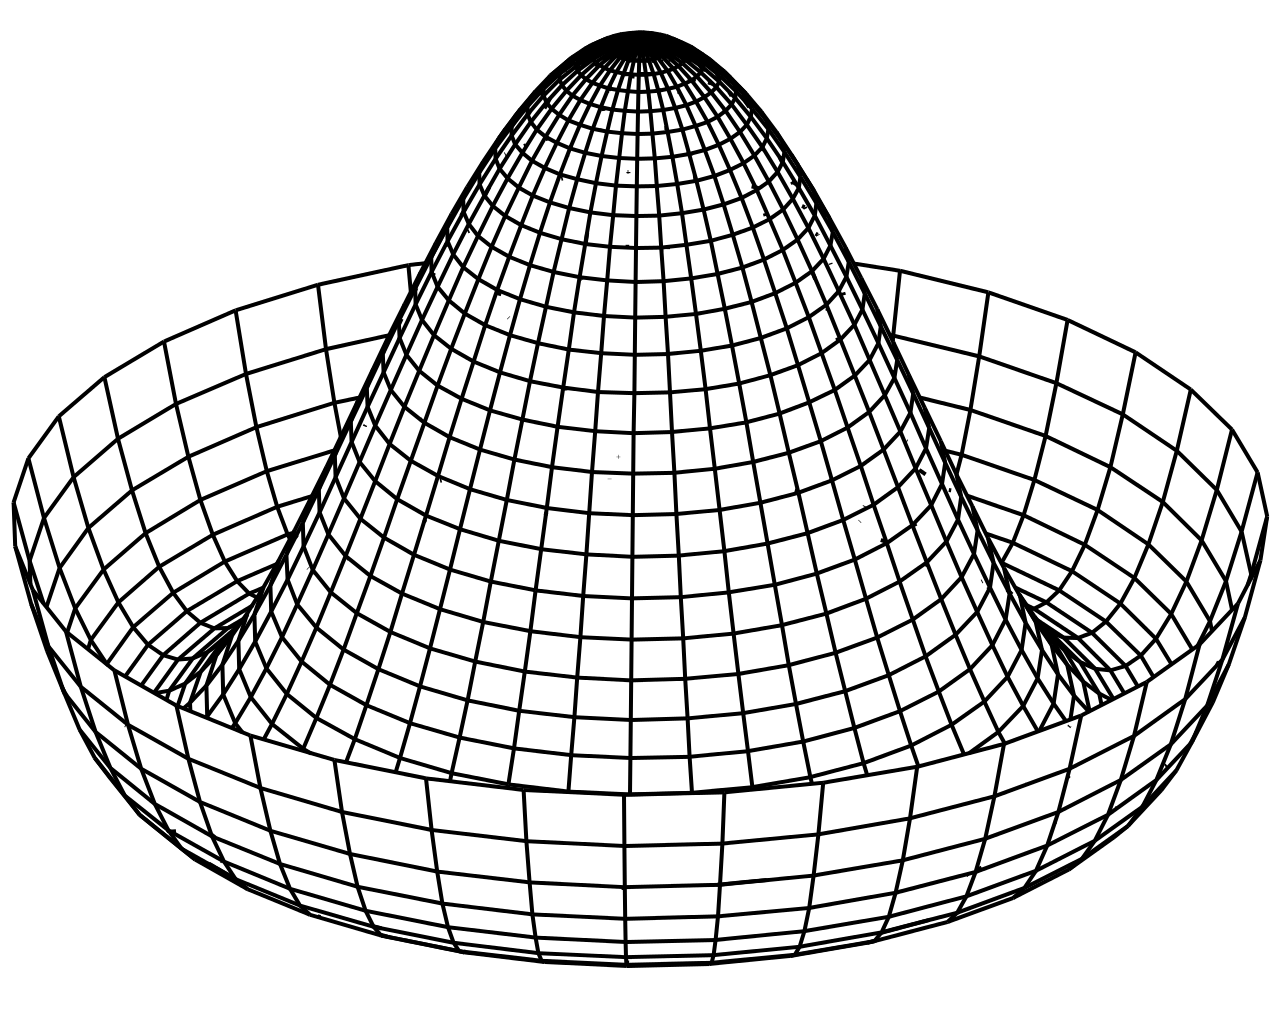
\includegraphics[width=.5\textwidth]{Lagrangian_Mechanics/mexican_hat.png}
                \caption{The ``Mexican Hat" potential. $U(\phi)=-10|\phi|^2+|\phi|^4.$}
                \label{fig:my_label}
            \end{figure}
        \end{frame}
        
        
    \subsection{Specific Results}
    
        \begin{frame}{Noether's Theorem}
        For a single particle, we can look at the momentum
            \[
            \mathbf{\dot{p}}_i=\frac{d}{dt}\frac{\partial \mathcal{L}}{\partial \mathbf{\dot{q}}_i}=\frac{\partial \mathcal{L}}{\partial \mathbf{q}_i}.
            \]
        If the Lagrangian does not depend on this coordinate then
            \[
            \implies \mathbf{\dot{p}}_i=\frac{d}{dt}\frac{\partial \mathcal{L}}{\partial \mathbf{\dot{q}}_i}=\frac{\partial \mathcal{L}}{\partial \mathbf{q}_i}=0.
            \]
        In other words, this generalized momentum is conserved!
        \end{frame}
        
        \begin{frame}{Noether's Theorem}
            \begin{theorem}[Emmy Noether]
                Every symmetry of a system corresponds to a conserved quantity.  In our case, every ignorable generalized coordinate corresponds to a conserved generalized momentum.
            \end{theorem}
        \end{frame}
        
        \begin{frame}{Noether's Theorem}
            \begin{example}
                Consider a central force field problem with $U(r)=\frac{1}{r}$. Choose polar coordinates so that $\mathbf{q}=(r(t),\theta(t)).$ Then
                \[
                \frac{\partial \mathcal{L}}{\partial r}=\frac{-1}{r^2}\quad \textrm{and}\quad \frac{d}{dt}\frac{\partial \mathcal{L}}{\partial \dot{r}}=\ddot{r}.
                \]
                Also,
                \[
                \frac{\partial \mathcal{L}}{\partial \theta}=0 \quad \implies\quad \frac{d}{dt}\frac{\partial \mathcal{L}}{\partial \dot{\theta}}=r\ddot{\theta}=0.
                \]
                Thus the E-L equations are
                \begin{align*}
                    \ddot{r}&=\frac{-1}{r^2}\\
                    \ddot{\theta}&=0.
                \end{align*}
            \end{example}
        \end{frame}
        
        \begin{frame}{Noether's Theorem}
            The fact that
            \[
            \ddot{\theta}=0
            \]
            means that \emph{angular momentum} is conserved.  
            
            \begin{remark}
            This is one of the huge upshots of the Lagrangian approach. Conserved quantities (=symmetries) are immediately obvious.  Modern physical theory relies heavily on symmetries.
            \end{remark}
        \end{frame}
        
        \begin{frame}{Applications}
            \begin{itemize}
                \item Classical mechanics.
                \item Classical field theory.
                \item Optics; Fermat's principle.
                \item Physical problems with constraints.
                \item Path integral formulation of quantum mechanics.
                \item General relativity; Optical paths, Einstein-Hilbert action.
            \end{itemize}
        \end{frame}
    
        
\end{document}